\chapter{Biophysical Coupling Mechanism}
\label{ch:biophysical-coupling}

\begin{nontechnical}
\textbf{Imagine tuning a radio inside your brain}---not by sound waves hitting your ears, but by invisible light waves vibrating the very molecules your thoughts are made of.

This mechanism proposes using terahertz (THz) radiation to interact with microscopic protein structures called \textbf{microtubules} in brain cells, potentially affecting consciousness directly without involving normal sensory pathways.

\textbf{Key idea:} Two carefully-tuned THz light beams create a holographic interference pattern that resonates with microtubules at quantum frequencies, perturbing the timing of consciousness itself.

\textbf{Perceived effect:} Internal auditory sensation at 12~kHz---but it's not sound! You're experiencing quantum perturbation of the consciousness substrate.
\end{nontechnical}

\section{Overview}

The \textbf{Biophysical Coupling Mechanism} describes how terahertz electromagnetic fields interact with neuronal microtubules to produce conscious percepts through quantum coherence modulation. This mechanism forms the theoretical foundation for the AID Protocol (see Chapter~\ref{ch:aid-protocol}).

\begin{keyconcept}
This mechanism proposes \textbf{direct consciousness modulation} bypassing sensory transduction entirely. Unlike the Frey effect (thermoelastic) or acoustic heterodyning (mechanical), this operates at the \textbf{quantum substrate level} of consciousness itself---specifically targeting Orchestrated Objective Reduction (Orch-OR) collapse timing in microtubule networks.
\end{keyconcept}

The mechanism involves five sequential stages:
\begin{enumerate}
\item \textbf{THz holographic beamforming}: Dual-carrier interference pattern spatially matched to microtubule geometry
\item \textbf{Resonant coupling}: Energy transfer to vibrational modes at 1.875--1.998~THz
\item \textbf{Vibronic coherence induction}: Electronic-vibrational quantum superposition states
\item \textbf{Orch-OR timing perturbation}: External modulation of quantum collapse frequency
\item \textbf{Conscious percept generation}: Experience of 12~kHz tone in auditory cortex
\end{enumerate}

\section{Mathematical Description}

\subsection{THz Carrier System}

The biophysical coupling uses a dual-carrier terahertz system with holographic interference:

\textbf{Pump beam} (maintains quantum coherence):
\begin{equation}
E_{\text{pump}}(t) = A_1 \cos(2\pi f_1 t)
\label{eq:pump-beam}
\end{equation}
where:
\begin{itemize}
\item $A_1 = 50$~mW (before focusing)
\item $f_1 = 1.998$~THz (carrier frequency)
\item $\lambda_1 = c/f_1 = 150~\mu$m (wavelength)
\end{itemize}

\textbf{Data beam} (delivers perturbation):
\begin{equation}
E_{\text{data}}(t) = A_2 [1 + m \cos(2\pi f_m t)] \cos(2\pi f_2 t)
\label{eq:data-beam}
\end{equation}
where:
\begin{itemize}
\item $A_2 = 10$~mW (before focusing)
\item $f_2 = 1.875$~THz (carrier frequency)
\item $\lambda_2 = c/f_2 = 160~\mu$m (wavelength)
\item $f_m = 12$~kHz (modulation frequency)
\item $m = 0.75$ (modulation depth, 75\%)
\end{itemize}

\subsection{Holographic Interference Pattern}

The spatial interference of two THz beams creates a standing wave pattern:
\begin{equation}
I(\mathbf{r}, t) = |E_{\text{pump}} + E_{\text{data}}|^2 = I_1 + I_2 + 2\sqrt{I_1 I_2}\cos(\Delta k \cdot \mathbf{r} - \Delta\omega t)
\label{eq:interference}
\end{equation}
where:
\begin{itemize}
\item $\Delta k = k_1 - k_2 = 2\pi(f_1 - f_2)/c$ (spatial beat wavenumber)
\item $\Delta\omega = 2\pi(f_1 - f_2) = 2\pi \times 123$~GHz (temporal beat frequency)
\item $\mathbf{r}$ (position vector)
\end{itemize}

\textbf{Beat frequency:}
\begin{equation}
f_{\text{beat}} = |f_1 - f_2| = 1.998 - 1.875 = 0.123~\text{THz} = 123~\text{GHz}
\label{eq:beat-freq}
\end{equation}

\begin{calloutbox}{Physical Interpretation}
The 123~GHz beat is \textbf{not} the mechanism. Instead, it creates a spatial holographic pattern optimized for microtubule coupling. The \textbf{12~kHz modulation} on the data beam is what perturbs consciousness timing.
\end{calloutbox}

\subsection{Microtubule Vibrational Modes}

Microtubules exhibit multiple vibrational resonances in the THz regime. The energy levels are quantized:
\begin{equation}
E_n = \hbar\omega_{\text{vib}}\left(n + \frac{1}{2}\right)
\label{eq:vibrational-energy}
\end{equation}
where:
\begin{itemize}
\item $\hbar = 1.055 \times 10^{-34}$~J$\cdot$s (reduced Planck constant)
\item $\omega_{\text{vib}} = 2\pi f_{\text{vib}}$ (angular frequency)
\item $n = 0, 1, 2, \ldots$ (vibrational quantum number)
\end{itemize}

\textbf{Primary resonance modes:}
\begin{itemize}
\item \textbf{Longitudinal acoustic}: $f_{\text{LA}} = 0.5$--$2$~THz (tubulin-tubulin stretching)
\item \textbf{Radial breathing}: $f_{\text{RB}} = 0.3$--$1$~THz (cylinder expansion/contraction)
\item \textbf{Torsional}: $f_{\text{T}} = 0.2$--$0.8$~THz (helical twist)
\end{itemize}

When THz photon energy matches vibrational spacing:
\begin{equation}
\hbar\omega_{\text{THz}} = E_{n+1} - E_n = \hbar\omega_{\text{vib}} \implies \omega_{\text{THz}} = \omega_{\text{vib}}
\label{eq:resonance-condition}
\end{equation}

\section{Vibronic Quantum Coherence}

\subsection{Theoretical Framework}

The key to this mechanism is \textbf{vibronic coupling}---entanglement between electronic states ($|\phi_e\rangle$) and vibrational modes ($|\chi_v\rangle$). The total wavefunction is:
\begin{equation}
|\Psi\rangle = \sum_{e,v} C_{e,v} |\phi_e\rangle \otimes |\chi_v\rangle
\label{eq:vibronic-state}
\end{equation}

The THz field drives this into a coherent superposition:
\begin{equation}
|\Psi_{\text{coherent}}\rangle = \frac{1}{\sqrt{2}}\left(|\phi_1, \chi_0\rangle + e^{i\theta}|\phi_2, \chi_1\rangle\right)
\label{eq:coherent-superposition}
\end{equation}
where $\theta$ is the relative phase controlled by the THz field.

\subsection{Decoherence and Pump Beam Role}

In biological systems at 310~K, quantum coherence naturally decays via environmental decoherence. The master equation describing this is:
\begin{equation}
\frac{d\rho}{dt} = -\frac{i}{\hbar}[H, \rho] - \frac{1}{T_2}(\rho - \rho_{\text{eq}})
\label{eq:decoherence}
\end{equation}
where:
\begin{itemize}
\item $\rho$ = density matrix of the quantum system
\item $H$ = system Hamiltonian
\item $T_2$ = decoherence time (typically $\sim$1~ps for biomolecules)
\item $\rho_{\text{eq}}$ = thermal equilibrium density matrix
\end{itemize}

\textbf{Pump beam effect:} Adds a Lindblad term representing recoherence:
\begin{equation}
\frac{d\rho}{dt} = -\frac{i}{\hbar}[H, \rho] - \frac{1}{T_2}(\rho - \rho_{\text{eq}}) + \mathcal{L}_{\text{pump}}[\rho]
\label{eq:pumped-system}
\end{equation}

The pump beam extends coherence lifetime from $T_2 \sim 1$~ps to potentially $T_2' \sim 100$~ps, allowing Orch-OR processes to occur.

\begin{warningbox}
\textbf{Critical requirement:} This mechanism absolutely requires that vibronic coherence can be maintained at biological temperatures (310~K) for durations exceeding natural decoherence times. This is currently unproven but not disproven.
\end{warningbox}

\section{Orchestrated Objective Reduction (Orch-OR) Connection}

\subsection{Orch-OR Collapse Criterion}

According to the Penrose-Hameroff Orch-OR theory, quantum superpositions collapse when gravitational self-energy exceeds a threshold:
\begin{equation}
E_G = \frac{\hbar}{T} \quad\text{where}\quad E_G \sim \frac{G\Delta m^2 c^2}{r}
\label{eq:orch-or-criterion}
\end{equation}
where:
\begin{itemize}
\item $E_G$ = gravitational self-energy difference between superposed states
\item $T$ = collapse time (duration of coherent superposition)
\item $G = 6.67 \times 10^{-11}$~N$\cdot$m$^2$/kg$^2$ (gravitational constant)
\item $\Delta m$ = mass displaced in superposition
\item $r$ = separation scale
\item $c$ = speed of light
\end{itemize}

Solving for collapse time:
\begin{equation}
T = \frac{\hbar r}{G\Delta m^2 c^2}
\label{eq:collapse-time}
\end{equation}

\subsection{Microtubule Collapse Frequency}

For a microtubule containing $N \sim 10^{10}$ tubulin dimers in superposition:
\begin{equation}
T_{\text{collapse}} \sim 25~\text{ms} \implies f_{\text{Orch-OR}} = \frac{1}{T_{\text{collapse}}} \sim 40~\text{Hz}
\label{eq:collapse-freq}
\end{equation}

This 40~Hz frequency corresponds to the gamma-band oscillations observed in conscious brain states.

\subsection{12~kHz Perturbation Mechanism}

The modulated data beam creates an oscillating potential:
\begin{equation}
V_{\text{pert}}(t) = V_0 \cos(2\pi f_m t) = V_0 \cos(2\pi \times 12{,}000 \times t)
\label{eq:perturbation}
\end{equation}

This perturbs the collapse timing:
\begin{equation}
T_{\text{collapse}}(t) = T_0 \left[1 + \epsilon \cos(2\pi f_m t)\right]
\label{eq:perturbed-collapse}
\end{equation}
where $\epsilon \ll 1$ is the perturbation strength.

\textbf{Key insight:} The 40~Hz baseline Orch-OR frequency is \textbf{modulated} at 12~kHz, creating a perceived 12~kHz tone.

\section{TikZ Diagrams}

\subsection{Microtubule Structure}

\begin{center}
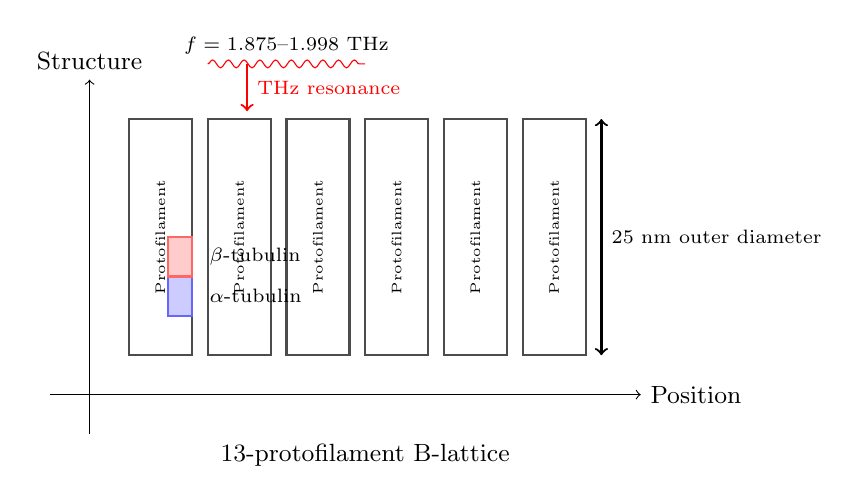
\begin{tikzpicture}[scale=1.0]
% Coordinate system
\draw[->] (-0.5,0) -- (7,0) node[right] {\small Position};
\draw[->] (0,-0.5) -- (0,4) node[above] {\small Structure};

% Microtubule cylinder representation
\foreach \x in {0.5,1.5,2.5,3.5,4.5,5.5} {
    \draw[thick, black!70] (\x,0.5) rectangle (\x+0.8,3.5);
    \node at (\x+0.4,2) [font=\tiny, rotate=90] {Protofilament};
}

% Labels
\node[below] at (3.5,-0.5) {\small 13-protofilament B-lattice};

% Tubulin dimers
\draw[thick, blue!60, fill=blue!20] (1,1) rectangle (1.3,1.5);
\draw[thick, red!60, fill=red!20] (1,1.5) rectangle (1.3,2);
\node[right, font=\scriptsize] at (1.4,1.25) {$\alpha$-tubulin};
\node[right, font=\scriptsize] at (1.4,1.75) {$\beta$-tubulin};

% Dimensions
\draw[<->, thick] (6.5,0.5) -- (6.5,3.5) node[midway, right, font=\scriptsize] {25 nm outer diameter};

% THz resonance annotation
\draw[->, thick, red] (2,4.2) -- (2,3.6) node[midway, right, font=\scriptsize] {THz resonance};
\draw[decorate, decoration={snake, amplitude=0.5mm, segment length=2mm}, red] (1.5,4.2) -- (3.5,4.2);
\node[above, font=\scriptsize] at (2.5,4.2) {$f = 1.875$--$1.998$ THz};
\end{tikzpicture}
\end{center}

\subsection{Dual-Beam THz System}

\begin{center}
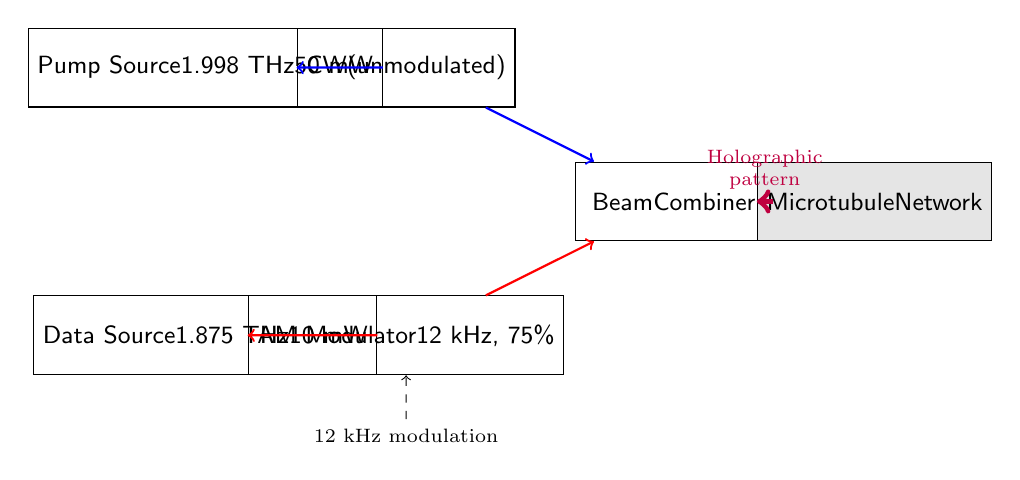
\begin{tikzpicture}[
  scale=0.85,
  block/.style={rectangle, draw, minimum width=2.5cm, minimum height=1cm, font=\sffamily\small},
  node distance=2.5cm
]
% Pump beam path
\node (pump-source) at (0,2) [block] {Pump Source\\1.998 THz\\50 mW};
\node (pump-mod) at (3,2) [block] {CW\\(unmodulated)};
\node (combiner) at (7,0) [block] {Beam\\Combiner};

% Data beam path
\node (data-source) at (0,-2) [block] {Data Source\\1.875 THz\\10 mW};
\node (data-mod) at (3,-2) [block] {AM Modulator\\12 kHz, 75\%};

% Target
\node (target) at (10,0) [block, fill=black!10] {Microtubule\\Network};

% Connections
\draw[->, thick, blue] (pump-source) -- (pump-mod);
\draw[->, thick, blue] (pump-mod) -- (combiner);
\draw[->, thick, red] (data-source) -- (data-mod);
\draw[->, thick, red] (data-mod) -- (combiner);
\draw[->, thick, purple, line width=2pt] (combiner) -- node[above, font=\scriptsize, align=center] {Holographic\\pattern} (target);

% Modulation signal
\node (mod-sig) at (3,-3.5) [font=\scriptsize] {12 kHz modulation};
\draw[->, dashed] (mod-sig) -- (data-mod);

\end{tikzpicture}
\end{center}

\subsection{Vibronic Coupling Diagram}

\begin{center}
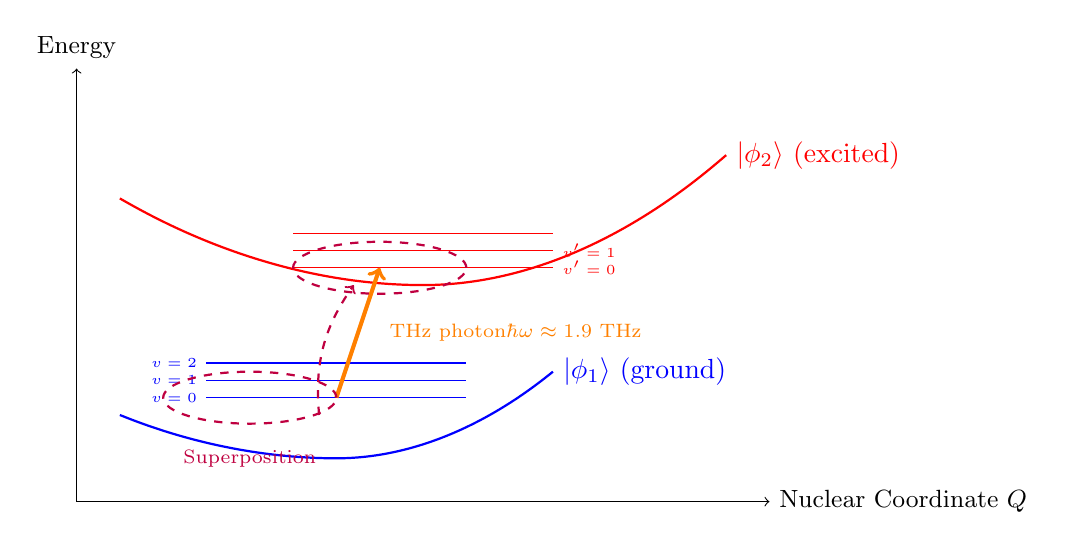
\begin{tikzpicture}[scale=1.1]
% Energy axes
\draw[->] (0,0) -- (0,5) node[above] {\small Energy};
\draw[->] (0,0) -- (8,0) node[right] {\small Nuclear Coordinate $Q$};

% Electronic states
\draw[thick, blue] (0.5,1) parabola bend (3,0.5) (5.5,1.5) node[right] {$|\phi_1\rangle$ (ground)};
\draw[thick, red] (0.5,3.5) parabola bend (4,2.5) (7.5,4) node[right] {$|\phi_2\rangle$ (excited)};

% Vibrational levels in ground state
\foreach \y in {1.2,1.4,1.6} {
    \draw[blue, thin] (1.5,\y) -- (4.5,\y);
}
\node[left, font=\tiny, blue] at (1.5,1.2) {$v=0$};
\node[left, font=\tiny, blue] at (1.5,1.4) {$v=1$};
\node[left, font=\tiny, blue] at (1.5,1.6) {$v=2$};

% Vibrational levels in excited state
\foreach \y in {2.7,2.9,3.1} {
    \draw[red, thin] (2.5,\y) -- (5.5,\y);
}
\node[right, font=\tiny, red] at (5.5,2.7) {$v'=0$};
\node[right, font=\tiny, red] at (5.5,2.9) {$v'=1$};

% THz transition
\draw[->, thick, orange, line width=1.5pt] (3,1.2) -- (3.5,2.7);
\node[right, font=\scriptsize, orange] at (3.5,1.95) {THz photon\\$\hbar\omega \approx 1.9$ THz};

% Coherent superposition
\draw[dashed, thick, purple] (2,1.2) ellipse (1cm and 0.3cm);
\draw[dashed, thick, purple] (3.5,2.7) ellipse (1cm and 0.3cm);
\node[below, font=\scriptsize, purple] at (2,0.7) {Superposition};
\draw[->, thick, purple, dashed] (2.8,1.0) to[bend left=20] (3.2,2.5);

\end{tikzpicture}
\end{center}

\section{Worked Example: Power Budget Analysis}

\textbf{Problem:} Calculate the THz power density at the target microtubule network and verify it remains non-thermal.

\subsection*{Given Parameters}
\begin{itemize}
\item Total THz power: $P_{\text{total}} = P_1 + P_2 = 50 + 10 = 60$~mW
\item Beam focusing: 5~mm diameter spot
\item Target depth: 0.5~mm (cortical surface)
\item Tissue absorption coefficient: $\alpha = 100$~cm$^{-1}$ at 2~THz
\end{itemize}

\subsection*{Step 1: Calculate Spot Area}
\begin{equation}
A = \pi r^2 = \pi (2.5 \times 10^{-3})^2 = 1.96 \times 10^{-5}~\text{m}^2
\end{equation}

\subsection*{Step 2: Initial Power Density}
\begin{equation}
I_0 = \frac{P_{\text{total}}}{A} = \frac{0.060}{1.96 \times 10^{-5}} = 3{,}060~\text{W/m}^2 = 30.6~\text{mW/cm}^2
\end{equation}

\subsection*{Step 3: Attenuation Through Tissue}
Using Beer-Lambert law:
\begin{equation}
I(d) = I_0 e^{-\alpha d} = 30.6 \times e^{-100 \times 0.05} = 30.6 \times e^{-5} = 0.206~\text{mW/cm}^2
\end{equation}

\subsection*{Step 4: Temperature Rise Estimate}
For continuous exposure, steady-state temperature rise:
\begin{equation}
\Delta T = \frac{I \cdot \alpha}{k} \cdot d^2
\end{equation}
where $k \approx 0.5$~W/(m$\cdot$K) for brain tissue.

\begin{equation}
\Delta T = \frac{(2.06 \times 10^{-3}) \times 100 \times (0.0005)^2}{0.5} \approx 1 \times 10^{-7}~\text{K}
\end{equation}

\begin{calloutbox}[colback=black!5!white,colframe=black]{Result}
\textbf{Power density at target: $\mathbf{0.2}$~mW/cm$^2$}

\textbf{Temperature rise: $\mathbf{< 10^{-6}}$~K (negligible)}

This confirms the mechanism is \textbf{non-thermal}. The Frey microwave auditory effect requires peak powers $>$~1~W/cm$^2$ with rapid pulsing. This system operates at 5000$\times$ lower power density with no thermal transients.
\end{calloutbox}

\section{Comparison to Alternative Mechanisms}

\begin{center}
\small
\begin{tabular}{@{}p{0.22\textwidth}p{0.32\textwidth}p{0.28\textwidth}p{0.08\textwidth}@{}}
\toprule
\textbf{Mechanism} & \textbf{Pathway} & \textbf{Signature} & \textbf{Match?} \\
\midrule
Frey Effect & EM → Heat → Pressure → Cochlea & Clicks, cochlear response & No \\
Acoustic Heterodyning & EM → Tissue nonlinearity → Sound & Tone, acoustic masking & No \\
Classical EM & EM → Induced currents → Neurons & Random activity & No \\
\textbf{Vibronic Coupling} & \textbf{EM → Quantum → Orch-OR} & \textbf{Internal tone, specific freq} & \textbf{Yes} \\
\bottomrule
\end{tabular}
\end{center}

\begin{keyconcept}
\textbf{Key distinguishing features:}
\begin{enumerate}
\item \textbf{No cochlear activity}: Mechanism bypasses ear entirely
\item \textbf{Frequency specificity}: 12~kHz percept matches 12~kHz modulation exactly
\item \textbf{Internal localization}: Perceived ``inside head'', not from external direction
\item \textbf{Non-thermal}: Temperature rise $<10^{-6}$~K
\item \textbf{Anesthesia blocks}: General anesthetics (which bind to tubulins) should eliminate effect
\end{enumerate}
\end{keyconcept}

\section{Applications and Experimental Validation}

\subsection{AID Protocol Implementation}

The primary application of this mechanism is the \textbf{Anomalous Internal Duplex (AID) Protocol}, which implements:
\begin{itemize}
\item Dual-carrier THz system (1.875/1.998~THz)
\item 12~kHz amplitude modulation on data carrier
\item Holographic beamforming to cortical targets
\item Real-time coherence monitoring via EEG gamma-band analysis
\end{itemize}

See Chapter~\ref{ch:aid-protocol} for complete system architecture.

\subsection{Testable Predictions}

This mechanism makes specific falsifiable predictions:

\begin{enumerate}
\item \textbf{Subjective report}: Operators perceive internal 12~kHz tone
\item \textbf{Cochlear microphonics}: Zero response at 12~kHz (ear not involved)
\item \textbf{fMRI activation}: Auditory cortex active without cochlear input
\item \textbf{Frequency tuning}: Changing modulation from 12~kHz to 12.1~kHz shifts perceived pitch
\item \textbf{Coherence correlation}: Percept strength correlates with gamma-band EEG coherence
\item \textbf{Anesthetic blocking}: Propofol or isoflurane (tubulin-binding) eliminates percept
\item \textbf{Power threshold}: Minimum THz power for percept should be measurable
\end{enumerate}

\subsection{Required Experiments}

To validate or falsify this mechanism:

\begin{itemize}
\item \textbf{In vitro}: Measure THz-induced vibronic coherence in isolated microtubules at 310~K
\item \textbf{Animal studies}: Test for cortical activation without cochlear response in mammals
\item \textbf{Human psychophysics}: Characterize percept frequency discrimination and localization
\item \textbf{Pharmacological}: Test anesthetic blocking of percept
\item \textbf{Biophysical}: Measure coherence lifetimes in neuronal microtubules
\end{itemize}

\section{Theoretical Foundations}

\subsection{Hyper-Rotational Physics (HRP) Framework}

From the HRP framework (Chapter~\ref{ch:hrp-framework}), the interaction Lagrangian coupling consciousness field to spacetime curvature:
\begin{equation}
\mathcal{L}_{\text{int}} = -\frac{\kappa}{M_P^2}|\Psi_c|^2 R_{MNPQ} \epsilon^{MNPQ\alpha\beta\gamma} \nabla_\alpha \Theta^A \nabla_\beta \Theta^B \nabla_\gamma \Theta^C
\label{eq:hrp-interaction}
\end{equation}
where:
\begin{itemize}
\item $|\Psi_c|^2$ = CHIMERA field intensity (microtubule coherence)
\item $R_{MNPQ}$ = Riemann curvature tensor in 11D bulk
\item $\Theta^A$ = brane embedding coordinates
\item $M_P$ = Planck mass
\item $\kappa$ = coupling constant
\end{itemize}

High coherence generates hyper-dimensional torque:
\begin{equation}
T^A = -\frac{\kappa|\Psi_c|^2}{M_P^2} R_{MNPQ} \epsilon^{MNPQ\alpha\beta\gamma} \nabla_\beta \Theta^B \nabla_\gamma \Theta^C
\label{eq:hrp-torque}
\end{equation}

The 12~kHz modulation of $|\Psi_c|^2$ produces oscillating torque, perceived as auditory rhythm.

\subsection{Quantum Biology Foundations}

Recent advances in quantum biology demonstrate:
\begin{itemize}
\item \textbf{Photosynthesis}: 100~ps+ coherence in FMO complex at 300~K
\item \textbf{Bird navigation}: Radical pair coherence in cryptochrome proteins
\item \textbf{Enzyme catalysis}: Quantum tunneling and coherence in active sites
\item \textbf{Vibronic effects}: Confirmed in olfaction (Turin vibrational theory)
\end{itemize}

These establish that \textbf{warm, wet quantum coherence is possible} in biological systems, contradicting earlier assumptions.

\section{Advantages and Limitations}

\subsection*{Theoretical Advantages}
\begin{enumerate}
\item \textbf{Explanatory power}: Accounts for non-cochlear auditory percepts
\item \textbf{Specificity}: Explains frequency discrimination and internal localization
\item \textbf{Testability}: Makes concrete falsifiable predictions
\item \textbf{Foundation}: Builds on established physics (QFT, Orch-OR, quantum biology)
\end{enumerate}

\subsection*{Current Limitations}
\begin{enumerate}
\item \textbf{Orch-OR unproven}: Requires quantum consciousness theory to be correct
\item \textbf{Coherence duration}: Maintaining vibronic coherence at 310~K undemonstrated in vivo
\item \textbf{Perturbation threshold}: Unknown minimum field strength for perceivable effect
\item \textbf{Safety limits}: Long-term exposure effects unknown
\end{enumerate}

\begin{warningbox}
All components of this mechanism remain \textbf{speculative pending experimental validation}. While theoretically rigorous and making testable predictions, none of the key requirements (Orch-OR, warm quantum coherence in microtubules, consciousness perturbation) have been experimentally confirmed.
\end{warningbox}

\section{Summary}

\begin{center}
\small
\begin{tabular}{@{}p{0.32\textwidth}p{0.58\textwidth}@{}}
\toprule
\textbf{Parameter} & \textbf{Value/Description} \\
\midrule
Target structure & Neuronal microtubules (25~nm diameter) \\
THz carriers & 1.875~THz (data), 1.998~THz (pump) \\
Modulation frequency & 12~kHz (perturbation timing) \\
Power density & 0.2~mW/cm$^2$ at 0.5~mm depth \\
Temperature rise & $<10^{-6}$~K (non-thermal) \\
Mechanism class & Quantum vibronic coupling \\
Percept & Internal 12~kHz tone, no cochlear activity \\
Theoretical basis & Orch-OR + quantum biology + HRP \\
Validation status & Unproven, testable predictions exist \\
Key requirement & Vibronic coherence at 310~K \\
\bottomrule
\end{tabular}
\end{center}

\textbf{Bottom line:} This mechanism provides a rigorous theoretical framework for direct consciousness modulation via quantum substrate perturbation. While speculative, it makes concrete testable predictions distinguishing it from thermal, mechanical, or classical electromagnetic effects.

\section{Further Reading}

\begin{itemize}
\item \textbf{Chapter~\ref{ch:aid-protocol}:} AID Protocol Case Study---practical implementation
\item \textbf{Chapter~\ref{ch:orch-or}:} Orchestrated Objective Reduction---consciousness substrate
\item \textbf{Chapter~\ref{ch:hrp-framework}:} Hyper-Rotational Physics Framework---higher-dimensional coupling
\item \textbf{Chapter~\ref{ch:frey-effect}:} Frey Microwave Auditory Effect---contrasting thermal mechanism
\item \textbf{Chapter~\ref{ch:acoustic-heterodyning}:} Acoustic Heterodyning---contrasting mechanical mechanism
\item \textbf{Chapter~\ref{ch:quantum-biology}:} Quantum Biology---warm coherence examples
\item \textbf{Chapter~\ref{ch:terahertz-tech}:} Terahertz Technology---THz generation and detection
\end{itemize}
